%%%%%%%%%%%%%%%%%%%%%%%%%%%%%%%%%%%%%%%%%
% Structured General Purpose Assignment
% LaTeX Template
%
% This template has been downloaded from:
% http://www.latextemplates.com
%
% Original author:
% Ted Pavlic (http://www.tedpavlic.com)
%
% Note:
% The \lipsum[#] commands throughout this template generate dummy text
% to fill the template out. These commands should all be removed when 
% writing assignment content.
%
%%%%%%%%%%%%%%%%%%%%%%%%%%%%%%%%%%%%%%%%%

\documentclass{article}

\usepackage{fancyhdr} % Required for custom headers
\usepackage{lastpage} % Required to determine the last page for the footer
\usepackage{extramarks} % Required for headers and footers
\usepackage{graphicx} % Required to insert images
\usepackage[utf8]{inputenc}

% Margins
\topmargin=-0.45in
\evensidemargin=0in
\oddsidemargin=0in
\textwidth=6.5in
\textheight=9.0in
\headsep=0.25in 

\linespread{1.1} % Line spacing



\setlength\parindent{0pt} % Removes all indentation from paragraphs

%----------------------------------------------------------------------------------------
%	DOCUMENT STRUCTURE COMMANDS
%	Skip this unless you know what you're doing
%----------------------------------------------------------------------------------------

% Header and footer for when a page split occurs within a problem environment
\newcommand{\enterProblemHeader}[1]{
\nobreak\extramarks{#1}{#1 continued on next page\ldots}\nobreak
\nobreak\extramarks{#1 (continued)}{#1 continued on next page\ldots}\nobreak
}

% Header and footer for when a page split occurs between problem environments
\newcommand{\exitProblemHeader}[1]{
\nobreak\extramarks{#1 (continued)}{#1 continued on next page\ldots}\nobreak
\nobreak\extramarks{#1}{}\nobreak
}

\setcounter{secnumdepth}{0} % Removes default section numbers
\newcounter{homeworkProblemCounter} % Creates a counter to keep track of the number of problems

%----------------------------------------------------------------------------------------
%	NAME AND CLASS SECTION
%----------------------------------------------------------------------------------------

\newcommand{\lessonNumber}[1]{Lezione\ \##1} % Assignment title
\newcommand{\lessonDate}[4]{#1,\ #2\ #3\ #4} % Due date
\newcommand{\lessonCourse}[1]{#1} % Course/class
\newcommand{\lessonTime}[1]{#1} % Class/lecture time
\newcommand{\lessonTeacher}[1]{#1} % Teacher/lecturer
\newcommand{\lessonAuthor}[1]{#1} % Your name
\begin{document}

\section{Verifica e validazione(12)}


\begin{itemize}

	\item \textbf{Verifica:} "ho fatto il sistema nel modo giusto", accerta che l'esecuzione delle attività di processi svolti nella fase in esame non abbia introdotto errori nel prodotto;
	\item \textbf{Validazione:} "ho fatto il sistema giusto", accerta che il prodotto realizzato sia conforme alle attese.

\end{itemize}

La \textit{software verification} ricerca la completezza e la correttezza del software e tratta ciò che lo supporta. Consente di valutare di conseguenza che il sw sia validato. La verifica è a supporto della validazione e la validazione è l'ultima cosa che faccio in un progetto. La verifica è un attività che svolgo durante \textbf{tutto lo sviluppo} fino all'ultimo istante dove farò validazione, che servirà a dire che ciò che ho fatto è la cosa giusta. La verifica va fatta per impedire che la risposta finale non sia sbagliata. Devo garantire tre cose importanti:

\begin{itemize}

	\item \textbf{Consistenza:} "sono ciò che vi attendevate fossi";
	\item \textbf{Correttezza:} "ciò che ho conseguito è corretto rispetto alle norme";
	\item \textbf{Completezza:} "tutto ciò che ho creato è tutto ciò era atteso".

\end{itemize}

Sono tre caratteristiche di cui devo accertare l'esistenza su tutti i prodotti parziali dello sviluppo. Il verificatore impara le norme e dice che quello che è stato fornito è fatto come richiesto. Non corregge nè rifà il lavoro ma controlla solo che tutto rispetti le tre caratteristiche. La validazione conseguentemente è una conferma \textbf{by examination}, mostra copertura dei requisiti (utente e sw).

Per il verificatore ho due forme di \textbf{analisi}:

\begin{itemize}

	\item \textbf{Analisi statica:} non richiede l'esecuzione del programma, studia le caratteristiche del codice sorgente (e a volte anche del codice oggetto), conformità a regole date, assenza di difetti, presenza di proprietà positive;
	\item \textbf{Analisi dinamica:} richiede l'esecuzione del programma, viene effettuata tramite \textbf{test}, usata sia nella verifica che nella validazione.						\begin{itemize}

			\item \textbf{Ripetibilità:} è un requisito essenziale. Dobbiamo assumere uno stato iniziale prima dell'esecuzione in quanto ha influenza sia diretta che indiretta sull'esecuzione. Il test deve essere \textbf{deterministico} ed eseguire le cose secondo un ordine noto. \textbf{Specifica di un test};
			\item \textbf{Strumenti}:
				\begin{itemize}

					\item \textbf{Driver:} componente attiva fittizia per pilotare una parte;
					\item \textbf{Stub:} componente passiva fittizia per simulare una parte;
					\item \textbf{Logger:} componente non intrusiva di registrazione dei dati di esecuzione per l'analisi dei risultati. Ogni tanto deve lasciare traccia del suo esito;	
	
				\end{itemize}
	\		item \textbf{Unità:} può essere anche un aggregato di procedure. La più piccola unità sw che è conveniente verificare singolarmente. Un \textit{modulo} è parte dell'unità, un \textit{componente} integra più unità.

		\end{itemize}

\end{itemize}

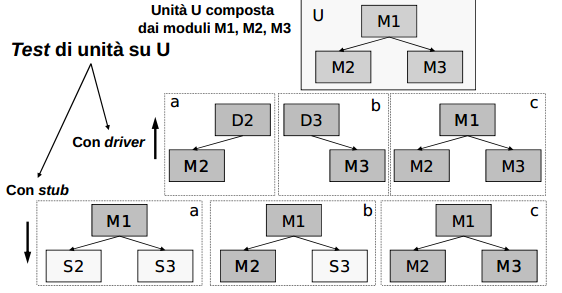
\includegraphics[width=0.5\columnwidth]{img3} % Example image

Con \textbf{stub} ho dei test \textit{Top down} dalla radice alle foglie, con \textbf{driver} ho dei test \textit{Bottom up} dalle foglie alla radice

Tipi di test

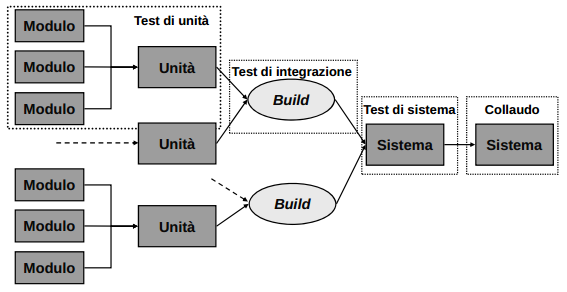
\includegraphics[width=0.5\columnwidth]{img4} % Example image

\begin{itemize}
	\item \textbf{Test di unità:} si svolgono con il massimo grado di parallelismo, la responsabilità è dello stesso programmatore sulle unità più piccole. L'obbiettivo è quello di verificare la correttezza del codice.
	\item \textbf{Test di integrazione:} le componenti vengono verificate e sviluppate in parallelo, rileva errori residui nella realizzazione dei componenti, cambiamenti nelle interfacce, requisiti, integrazione con altre applicazioni non ben conosciute.
	\item \textbf{Test di sistema e collaudo:} dai requisiti so dire quanti test di sistema avrò. I test di sistema è un'attività interna del fornitore per accertare la copertura dei requisiti, il collaudo invece viene supervisionato dal committente.
	\item \textbf{Test di regressione:} è l'insieme dei test che accertano che la modifica di una parte P non causi problemi in P o in altre parte che dipendono da essa, infatti modifiche aggiunte o rimozioni non devono pregiudicare le funzionalità già verificate.
\end{itemize}

\subsection{Analisi Statica}
Si può applicare ai metodi di lettura che si possono suddividere in due tipi:
\begin{itemize}
	\item \textbf{Walkthrought:} l'obbiettivo è quello di rilevare la presenza di difetti, si esegue una lettura a largo spetto senza l'assunzione di presupposti, le fasi sono: pianificazione, lettura, discussione, correzione dei difetti. 
	\item \textbf{Inspection:} l'obbiettivo è sempre quello di rilevare difetti ma eseguendo una lettura mirata, si focalizza la ricerca su presupposti, le fasi sono: pianificazione, definizione della lista di controllo, lettura, correzione dei difetti.
\end{itemize}

\textit{Inspection} è basato su errori presupposti ed è più rapido, \textit{Walkthrought} richiede maggiore attenzione ma è più collaborativo.

Valori dell'\textbf{Analisi Statica}:

\begin{itemize}
	\item \textbf{Funzionalità:} analisi statica come attività preliminare, liste di controllo rispetto ai relativi requisiti \textit{(tutte e solo le funzionalità per tutti e solo i componenti necessari, compatibilità tra tutte le soluzioni adottate)}, valutazione di accuratezza;
	\item \textbf{Affidabilità:} dimostrabile tramite combinazione di prove, analisi statica come attività preliminare, liste di controllo rispetto ai relativi requisiti \textit{(robustezza, capacità di ripristino e recupero da errori, adesione alle norme)}, valutazione di maturità.
	\item \textbf{Usabilità:} le prove sono imprescindibili, analisi statica come attività complementare, liste di controllo rispetto ai manuali d'uso \textit{(comprensibilità, apprendibilità, adesione a norme e prescrizioni)}, questionari sottomessi agli utenti.
	\item \textbf{Efficenza:} le prove sono necessarie, analisi statica come attività complementare, liste di controllo rispetto alle norme di codifica, margini di miglioramento e confidenza grazie alla confidenza acquisita.
	\item \textbf{Manutenibità:} analisi statica come strumento ideale, liste di controllo rispetto a specifiche norme di codifica, e alla prove per accertarne, prove di stabilità.
	\item \textbf{Portabilità:} analisi statica come strumento ideale, liste di controllo rispetto a specifiche norme di codifica, prove come strumento complementare.
\end{itemize}

Con un software di grandi dimensioni si deve stare attenti alla sicurezza intesa come \textbf{safety}, prevenzione di condizioni di pericolo a persone o cose, e come \textbf{security}, prevenzione di intrusioni. Sw così complessi devono possedere tutte le funzionalità, specificate nei requisiti e tutte le caratteristiche non funzionali per garantire che il sistema lavori sempre come previsto.\\
Nessun linguaggio di programmazione garantisce a priori la completa verificabilità di ogni programma scritto con esso.\\

Tecniche di verifica:
\begin{itemize}
	\item \textbf{Tracciamento:} dimostrare complettezza ed economicità della soluzione \textit{(soddisfacimento di tutti i requisiti, nessuna funzionalità superflua, nessun componente ingiustificato)}, questo va fatto tra i requisiti software e i requisiti utente, tra sorgente e codice oggetto, tra procedure di verifica e requisiti.\\
	Particolari stili di codifica facilitano la verifica mediante tracciamento \textit{assegnare singoli requisiti a singoli moduli del programma così da avere una sola procedura di prova, maggiorare l'astrazione}.
	\item \textbf{Revisioni:} strumento essenziale del processo di verifica, non sono automatizzabili, possono essere formali \textbf{audit} o informali \textbf{joint review}

\end{itemize}

Tipi di analisi statica:
\begin{enumerate}
	\item \textbf{Flusso di controllo:} si accerta che il codice si esegua nella sequenza specificata, che sia ben strutturato e identifica eventuali segmenti di codice che non terminano, non sono raggiungibili;
	\item \textbf{Flusso dei dati:} rileva possibili anomalie e accerta che nessun cammino di esecuzione porti ad uno stato incongruente;
	\item \textbf{Flusso dell'informazione:} determinare le dipendenze in ingresso, uscita, le sole consentite sono quelle previste nella specifica;
	\item \textbf{Esecuzione simbolica:} si verificano le proprietà del programma tramite la manipolazione algebrica del codice sorgente \textit{(lo si esegue facendo sostituzioni inverse)};
	\item \textbf{Verifica formale del codice:} provare la correttezza del codice sorgente rispetto alla specifica algebrica dei requisiti, si verifica la correttezza parziale;
	\item \textbf{Verifica del limite:} verificare che i dati del programma restino entro i limiti del loro tipo e dalla precisione desiderata;
	\item \textbf{Uso dello stack:} si determina la massima domanda di stack richiesta da un'esecuzione in relazione con la dimensione dell'area di memoria, verificare che non ci possa essere collisione tra stack e heap;
	\item \textbf{Comportamento temporale:} attenzione alle proprietà temporali richieste dalle dipendenze delle uscite dagli ingressi del programma;
	\item \textbf{Interferenza:} controllare l'assenza di interferenze tra le partizioni separate del sistema;
	\item \textbf{Codice oggetto:} assicurarsi che il codice oggetto sia una traduzione esatta del codice sorgente, che non ci siano errori o omissioni introdotte dal compilatore.
\end{enumerate}
La verifica solo retrospettiva \textit{(a valle dello sviluppo)} è spesso inadeguata.
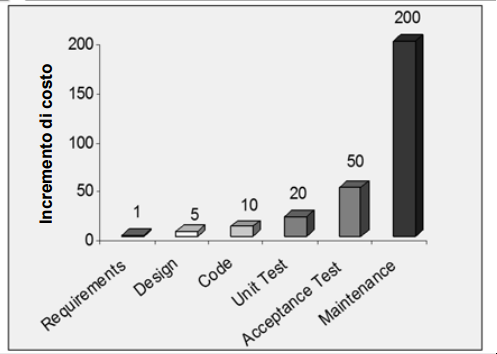
\includegraphics[width=0.5\columnwidth]{img5} % Example image

Eseguire cicli revisione, verifica dopo ogni rilevazione d'errore è troppo oneroso, meglio effettuare analisi statiche durante la codifica. Si deve cercare di avere delle linee guida per la codifica del codice come prediligere o proibire l'uso di particolari costrutti, \textit{separare le interfacce dall'implementazione, massimizzare l'implementazione, massimizzare l'incapsulazione, usare tipi specializzati per specificare i dati}.

\subsection{Analisi Dinamica}

Analisi dinamica=test, la prova che consiste nella verifica dinamica del comportamento del programma, queste prove si faranno su un insieme finito di casi selezionati nel dominio delle esecuzioni possibili.\\

classificazione delle problematiche:

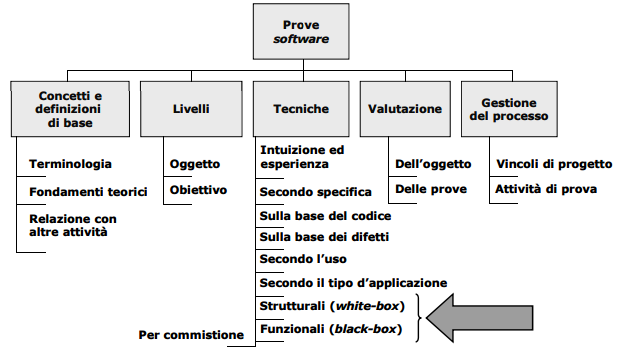
\includegraphics[width=0.5\columnwidth]{img6} % Example image

Dentro la classificazione ci deve essere:

\begin{itemize}
	\item Terminologia, Fault \rightarrow Error \rightarrow Failure
	\begin{itemize}
		\item \textbf{Failure:} quando il comportamento del sistema devia da quello che ci si aspetta;
		\item \textbf{Error:} possono essere meccanici, di algoritmo o concettuali e causano guasti \textit{Fault} terminali;
		\item \textbf{Fault:} sono quelli che fanno si che esista l'errore.
	\end{itemize}
	\item Fondamenti teorici;
	\item Oggetti delle prove;
	\item Obbiettivi delle prove: installazione nell'ambiente di prova, accettazione, collaudo;
	\item Vincoli di progetto: definizione del processo dei prodotti e del personale addetto alle prove, stima e controllo dei costi;
	\item Attività di prova: pianificazione e specifica dei casi di prova, sviluppo ambiente di prova.
\end{itemize}



\end{document}